\documentclass[border=10pt]{standalone}
\usepackage{pgfplots}
\pgfplotsset{compat=1.18}
\begin{document}
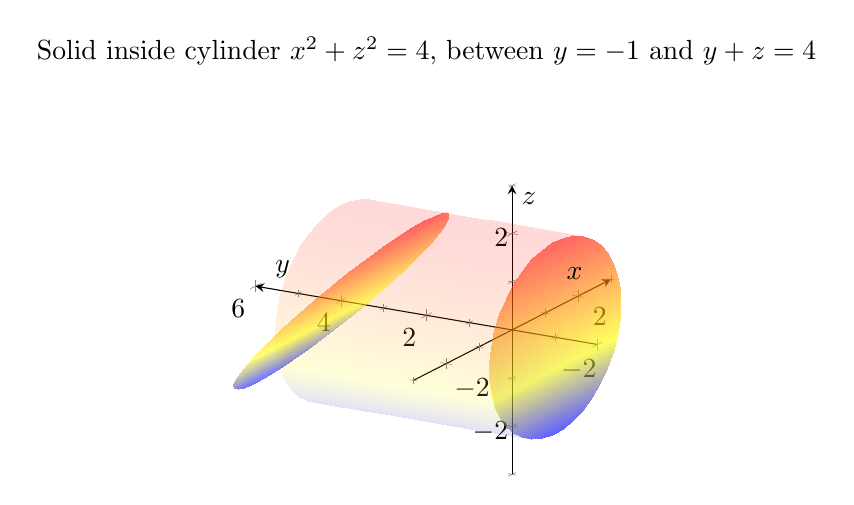
\begin{tikzpicture}
\begin{axis}[
    view={-60}{22},
    xlabel={$x$}, ylabel={$y$}, zlabel={$z$},
    xmin=-3, xmax=3, ymin=-2, ymax=6, zmin=-3, zmax=3,
    grid=both, minor tick num=1,
    title={Solid inside cylinder $x^2+z^2=4$, between $y=-1$ and $y+z=4$},
    axis lines=middle
]
% Cylindrical lateral surface (transparent blue)
\addplot3[
    surf, shader=interp, opacity=0.15, samples=40, samples y=20,
    domain=0:360, domain y=-1:4,
    z buffer=sort
] (
    {2*cos(x)},
    {y},
    {2*sin(x)}
);

% Bottom face y = -1 (red)
\addplot3[
    surf, shader=interp, opacity=0.55, samples=40, samples y=20,
    domain=0:360, domain y=0:2, z buffer=sort
] (
    {y*cos(x)},
    {-1},
    {y*sin(x)}
);

% Top face y = 4 - z (green)
\addplot3[
    surf, shader=interp, opacity=0.55, samples=40, samples y=20,
    domain=0:360, domain y=0:2, z buffer=sort
] (
    {y*cos(x)},
    {4 - y*sin(x)},
    {y*sin(x)}
);
\end{axis}
\end{tikzpicture}
\end{document}